\documentclass[areasetadvanced]{scrartcl}

\usepackage[utf8]{inputenc}
\usepackage[T2A]{fontenc}
\usepackage[english,russian]{babel}

\usepackage[footskip=1cm,left=25mm, right=15mm, top=20mm, bottom=20mm]{geometry}
\usepackage{setspace}
\usepackage{amsmath, amssymb} 
\usepackage{graphicx}
\usepackage{tikz}
\usetikzlibrary{arrows.meta}
\usepackage{float}
\usepackage{dashrule}
\usepackage{fancyhdr} 
\usepackage{hyperref} 
\usepackage{parskip}
\usepackage{textcomp, enumitem}
\usepackage{indentfirst}
\usepackage{graphicx}
\usepackage{algorithm}
\usepackage{algpseudocode}
\usepackage{array} 
\usepackage{geometry}
\usepackage{afterpage}
\usepackage{minted}
\setcounter{secnumdepth}{3} 
\setcounter{tocdepth}{3}    
\usepackage{listings} 

\newcommand{\icon}[1]{\includegraphics[height=1.2em]{#1}}

\tikzstyle{block} = [rectangle, rounded corners, minimum width=3cm, minimum height=1cm, text centered, draw=black, fill=lightgray]

\setkomafont{sectioning}{\normalfont\bfseries} 
\setkomafont{section}{\normalfont\Large\bfseries}
\setkomafont{subsection}{\normalfont\large\bfseries}
\setkomafont{subsubsection}{\normalfont\large\bfseries}
\setkomafont{paragraph}{\normalfont\large\bfseries} 

\lstset{
  language=Haskell,
  basicstyle=\ttfamily\small,
  keywordstyle=\color{blue}\bfseries,
  stringstyle=\color{red},
  commentstyle=\color{green!70!black},
  numbers=left,
  numberstyle=\tiny,
  stepnumber=1,
  numbersep=10pt,
  showstringspaces=false,
  breaklines=true,
  frame=single
}

\lstdefinelanguage{Lua}{
    keywords={function, end, if, then, else, elseif, for, while, do, repeat, until, break, return, local, and, or, not, true, false, nil},
    keywordstyle=\color{blue}\bfseries,
    stringstyle=\color{red},
    commentstyle=\color{green!70!black},
    morestring=[s]{"}{"},
    morestring=[s]{'}{'},
    morecomment=[l]{--},
    morecomment=[s]{--[[}{]]},
    basicstyle=\ttfamily\small,
    numbers=left,
    numberstyle=\tiny,
    stepnumber=1,
    numbersep=10pt,
    showstringspaces=false,
    breaklines=true,
    frame=single
}

\setlength{\parindent}{1.25cm}
\setcounter{tocdepth}{2}
\begin{document}
\sloppy
	\thispagestyle{empty}
	\begin{center}
		\large{МИНОБРНАУКИ РОССИИ} \par
		\vspace{0.3cm}
		\normalsize
		{ФЕДЕРАЛЬНОЕ ГОСУДАРСТВЕННОЕ АВТОНОМНОЕ ОБРАЗОВАТЕЛЬНОЕ УЧРЕЖДЕНИЕ ВЫСШЕГО ОБРАЗОВАНИЯ} \par
		\vspace{0.3cm}
		\textbf{\guillemotleft САНКТ-ПЕТЕРБУРГСКИЙ ПОЛИТЕХНИЧЕСКИЙ}
		\textbf{УНИВЕРСИТЕТ ПЕТРА ВЕЛИКОГО\guillemotright} \par
		\vspace{0.3cm}
		{Институт компьютерных наук и кибербезопасности}\par
		{Высшая школа технологий искусственного интеллекта}\par
	\end{center}
	\vfill
	\begin{center}
		{\huge Реферат по дисциплине}\par
        {\huge \guillemotleft Управление прроектами\guillemotright}
		
		\Huge \guillemotleft Стадии проектирования автоматизированных информационных систем\guillemotright
         
	\end{center}
	\vfill
	\begin{flushleft}
		Студент: \hspace{1.8cm} \rule[0pt]{2.5cm}{0.5pt}\hfill Салимли Айзек Мухтар Оглы\par
		\vspace{1.5cm}
		Преподаватель: \hspace{0.55cm} \rule[0pt]{2.5cm}{0.5pt}\hfill  Большаков Александр Афанасьевич
	\end{flushleft}
	\vspace{0.5cm}
	\begin{flushright}
		\guillemotleft \rule[0pt]{0.8cm}{0.5pt}\guillemotright \rule[0pt]{2cm}{0.5pt} 20\rule[0pt]{0.5cm}{0.5pt} г.
	\end{flushright}
	\vfill
	\begin{center}
		Санкт-Петербург, 2025
	\end{center}
	\newpage
	\tableofcontents
	\newpage
\section*{Введение}
	\addcontentsline{toc}{section}{Введение}


Автоматизированная информационная система (АИС) — это комплекс, включающий программное обеспечение, аппаратные средства, и данные, объединенные для сбора, обработки, хранения и выдачи информации в рамках конкретной предметной области. Основная цель АИС — повышение эффективности управления и поддержки бизнес-процессов.

    Современные АИС создаются в условиях быстро меняющихся требований и интеграции с чужими системами.
 
    Классические подходы (сверху-вниз/снизу-вверх, процессный/структурный) эффективны для локальных задач, но хуже адаптируются к изменениям.

    Подход на основе метамоделей повышает гибкость за счёт описания на более высоком уровне абстракции и согласованного изменения слоёв данных/логики/интерфейса.
\newpage
\section{Принципы организации проектирования АИС}

\subsection{Системное мышление и поэтапность работ}

Системное мышление в контексте проектирования информационных систем (АИС) предполагает интеграцию различных аспектов работы: от анализа потребностей до внедрения системы в эксплуатацию. Каждое решение в процессе проектирования должно быть принято с учётом всех взаимосвязанных факторов. Это позволяет создавать систему, которая будет работать как единое целое, а не как совокупность отдельных решений.

Процесс проектирования всегда разбивается на несколько этапов, что даёт возможность детально проработать каждый элемент системы и снизить риски. Подход поэтапного проектирования включает в себя анализ, проектирование, верификацию, тестирование и внедрение. Такой подход позволяет гибко адаптироваться к изменениям на каждом из этапов и учитывать реальные потребности бизнеса и заказчика.

\subsection{Разделение на слои: данные, логика, интерфейс и их согласованность}

Проектирование АИС часто включает разделение на несколько слоёв — данные, логика, и интерфейс. Каждый слой представляет собой отдельную подсистему, решающую свою задачу, но при этом все они должны быть согласованы между собой. Это ключевой момент, поскольку согласованность между слоями обеспечивает стабильность работы системы в целом.  

\begin{itemize}
    \item \textbf{Слой данных} включает в себя модели данных, базы данных и связанные с ними процессы обработки данных.
    \item \textbf{Слой логики} включает в себя бизнес-логику и алгоритмы, которые должны обеспечивать выполнение всех операций системы.
    \item \textbf{Слой интерфейса} представляет собой взаимодействие пользователя с системой, будь то графический интерфейс или интерфейсы взаимодействия с другими системами.
\end{itemize}

Обеспечение согласованности между этими слоями позволяет системе быть гибкой и легко адаптируемой к изменениям, поскольку изменение одного слоя должно минимально затрагивать другие.

\subsection{Фокус на изменяемость предметной области и интеграцию}

Очень важным аспектом проектирования АИС является способность системы адаптироваться к изменяющимся требованиям предметной области и возможности интеграции с внешними системами. В условиях быстро меняющегося рынка, где появляются новые требования и технологии, система должна быть гибкой и адаптируемой.  

Процесс проектирования должен учитывать возможности для добавления новых функциональностей или изменения существующих без значительных затрат на переработку всей системы. Также важно предусмотреть интеграцию с уже существующими системами и внешними сервисами, чтобы избежать избыточных затрат и повысить эффективность.


\begin{figure}[H]
	\centering
	\includegraphics[width=0.7\textwidth]{images/image copy 2.png}
	\caption{Схема принципов и планирования.}
\end{figure}


\newpage
\section{Этапы проектирования АИС}

\subsection{Содержательное описание объекта и процессов}

На начальном этапе проектирования важно правильно описать объект автоматизации и процессы, которые будут в ней отражены. Это описание является основой для дальнейшей работы и включает в себя подробное представление бизнес-процессов, требований заказчика и особенностей работы самой системы.

Данный этап предполагает не только изучение предметной области, но и анализ существующих систем, изучение их сильных и слабых сторон. Важно собрать всю необходимую информацию, которая поможет в дальнейшем процессе разработки.

\subsection{Формализованная схема / математическая модель}

После того как были собраны все необходимые данные и требования, создаётся формализованная схема или математическая модель системы. Эта модель позволяет чётко определить все связи между компонентами системы и процессы, которые в ней будут реализованы.  

Математические модели играют важную роль, так как позволяют протестировать систему на этапе проектирования. С помощью таких моделей можно заранее определить возможные проблемы, оценить эффективность предложенных решений и провести оптимизацию.

\subsection{ТЗ на систему и подсистемы: пилот-проект и внедрение}

Следующим этапом является создание технического задания (ТЗ) на систему и её подсистемы. Это документ, который чётко определяет, что должно быть реализовано в системе, какие функции она должна выполнять и какие требования предъявляются к её производительности, безопасности и устойчивости.

После разработки ТЗ приступают к созданию пилотного проекта — прототипа системы. Пилот позволяет протестировать систему в реальных условиях и выявить возможные ошибки или недочёты. На основе результатов тестирования пилота вносятся коррективы, после чего система внедряется в эксплуатацию.
\newpage
\begin{figure}[H]
	\centering
	\includegraphics[width=0.7\textwidth]{images/Screenshot 2025-10-15 at 11.13.40.png}
	\caption{Диаграмма этапов}
\end{figure}


\newpage
\section{Классический подход / метамодель}

\subsection{Классика: локальные решения, дорогие изменения схем данных}

Классический подход к проектированию АИС основывается на создании локальных решений, каждый из которых решает свою задачу. Это решение может быть простым и эффективным для определённого набора задач, однако оно часто ограничивает гибкость системы. Одним из недостатков классического подхода является высокая стоимость изменений в структуре данных, так как любые изменения на одном уровне системы могут потребовать переработки и других её частей.


\begin{figure}[H]
	\centering
	\includegraphics[width=0.7\textwidth]{images/image copy 5.png}
	\caption{Классический подход}
\end{figure}


\subsection{Метамодель: гибкость и переиспользование}

Метамодельный подход позволяет описывать систему на более высоком уровне абстракции. Вместо того чтобы разрабатывать каждое решение отдельно, создаются метамодели, которые описывают не только саму систему, но и её основные компоненты, а также их взаимосвязи. Это даёт возможность:
\begin{itemize}
    \item Гибко реагировать на изменения в требованиях.
    \item Переиспользовать компоненты для различных проектов.
    \item Легче интегрировать новые технологии и решения.
\end{itemize}

Метамодели включают в себя:
\begin{itemize}
    \item \textbf{Метаданные} — данные о данных, которые описывают их структуру и логику.
    \item \textbf{Металогика} — описание логики работы системы на более высоком уровне абстракции.
    \item \textbf{Мета-интерфейсы} — интерфейсы, которые обеспечивают взаимодействие между различными компонентами системы, при этом эти интерфейсы могут быть адаптированы или изменены с минимальными затратами.
\end{itemize}

\newpage
\section{Роли и артефакты}

\subsection{Единая терминология и модели: Заказчик $\rightarrow$ проектировщик $\rightarrow$ разработчик}

Процесс проектирования требует четкой согласованности терминологии и моделей между всеми участниками проекта. Заказчик, проектировщик и разработчик должны использовать единую терминологию, чтобы избежать недопонимания и ошибок в процессе разработки.

\begin{itemize}
    \item \textbf{Заказчик} формулирует требования к системе.
    \item \textbf{Проектировщик} разрабатывает архитектуру системы и её функциональные характеристики.
    \item \textbf{Разработчик} реализует систему в соответствии с архитектурой и требованиями.
\end{itemize}

\subsection{Артефакты: Модели требований, Архитектуры, Сценарии поведения}

Во время проектирования создаются различные артефакты, которые являются результатами работы на каждом этапе:

\begin{itemize}
    \item \textbf{Модели требований} описывают, какие функции и задачи должна выполнять система.
    \item \textbf{Архитектуры} системы — это её структура, включающая все компоненты и их взаимодействия.
    \item \textbf{Сценарии поведения} — это детализированные описания того, как система должна реагировать на различные входные данные и взаимодействие с пользователями.
\end{itemize}

\begin{figure}[H]
	\centering
	\includegraphics[width=0.7\textwidth]{images/image copy 6.png}
	\caption{Артефакты процесса управления}
\end{figure}


\newpage
\section{Стандарты жизненного цикла АИС: ISO/IEC 12207 и ISO/IEC 15288}

\subsection{ISO/IEC 12207 (ПО)}

Этот стандарт описывает процессы, которые должны быть выполнены при разработке программного обеспечения. Он делится на несколько категорий процессов:

\begin{itemize}
    \item \textbf{5 основных процессов:}
    \begin{itemize}
        \item \textbf{Заказ:} определение требований и планирование.
        \item \textbf{Поставка:} внедрение и настройка ПО.
        \item \textbf{Разработка:} создание и тестирование программного обеспечения.
        \item \textbf{Эксплуатация:} использование ПО в реальных условиях.
        \item \textbf{Сопровождение:} поддержка и развитие системы после её внедрения.
    \end{itemize}
    \item \textbf{4 организационных процесса:}  
    \begin{itemize}
        \item Управление проектом, инфраструктура, совершенствование процессов и обучение.
    \end{itemize}
    \item \textbf{8 вспомогательных процессов:}  
    \begin{itemize}
        \item Включает в себя документацию, управление конфигурацией, контроль качества, верификацию и аттестацию, аудит и решение проблем.
    \end{itemize}
\end{itemize}

\begin{figure}[H]
	\centering
	\includegraphics[width=0.7\textwidth]{images/image copy 3.png}
	\caption{Диаграмма стандарта ISO-12207}
\end{figure}

\subsection{ISO/IEC 15288 (Системы)}

Этот стандарт охватывает более широкий спектр, чем 12207, так как включает в себя процессы, связанные с проектированием и жизненным циклом сложных систем (не только ПО). Он разделяется на несколько групп процессов, включая технические, проектные и обеспечивающие процессы.

\begin{itemize}
    \item \textbf{Группы процессов:}
    \begin{itemize}
        \item \textbf{Соглашение (приобретение, постановка)}
        \item \textbf{Обеспечивающие на уровне предприятия}
        \item \textbf{Проектные (планирование, риски, конфигурация)}
        \item \textbf{Технические (требования, архитектура, реализация, интеграция, вериф./валидация, эксплуатация, сопровождение, списание)}
    \end{itemize}
\end{itemize}

\begin{figure}[H]
	\centering
	\includegraphics[width=0.7\textwidth]{images/image copy 4.png}
	\caption{Диаграмма стандарта ISO-15288}
\end{figure}

\newpage
\section{Примеры из реальной жизни}

\subsection{ERP-внедрение | ОАО «Тагмет» (SAP R/3)}

Внедрение ERP-системы на базе SAP R/3 на ОАО «Тагмет» показало высокие затраты и длительный процесс адаптации системы под специфику конкретного предприятия. Адаптация ERP-системы требует серьёзных усилий по настройке и изменению её функционала, что может занять месяцы. Это доказывает, что для специфических предприятий целесообразно разрабатывать собственные АСУ, которые будут более гибкими в адаптации и соответствовать потребностям бизнеса.

\subsection{Авиационная отрасль}

В авиационной отрасли на ранних стадиях проектирования часто выявляются дефекты, которые можно было бы избежать, если бы использовались более продвинутые подходы к моделированию. Использование архитектурных моделей, например, на AADL, и проведение анализа безопасности помогает значительно улучшить проект, выявляя возможные уязвимости ещё до того, как система будет построена. Это подтверждает важность верификации на стадии проектирования и моделирования.

\newpage
\section{ПО для проектирования АИС}

\subsection{Визуальное моделирование}

Для проектирования АИС широко используются инструменты визуального моделирования, такие как \textbf{IBM Rhapsody}, \textbf{Sparx EA}, \textbf{Modelio}, \textbf{Eclipse Papyrus}. Эти инструменты позволяют строить модели, использовать стандарты SysML/UML для представления архитектуры системы и её компонентов.  
\begin{figure}[H]
	\centering
	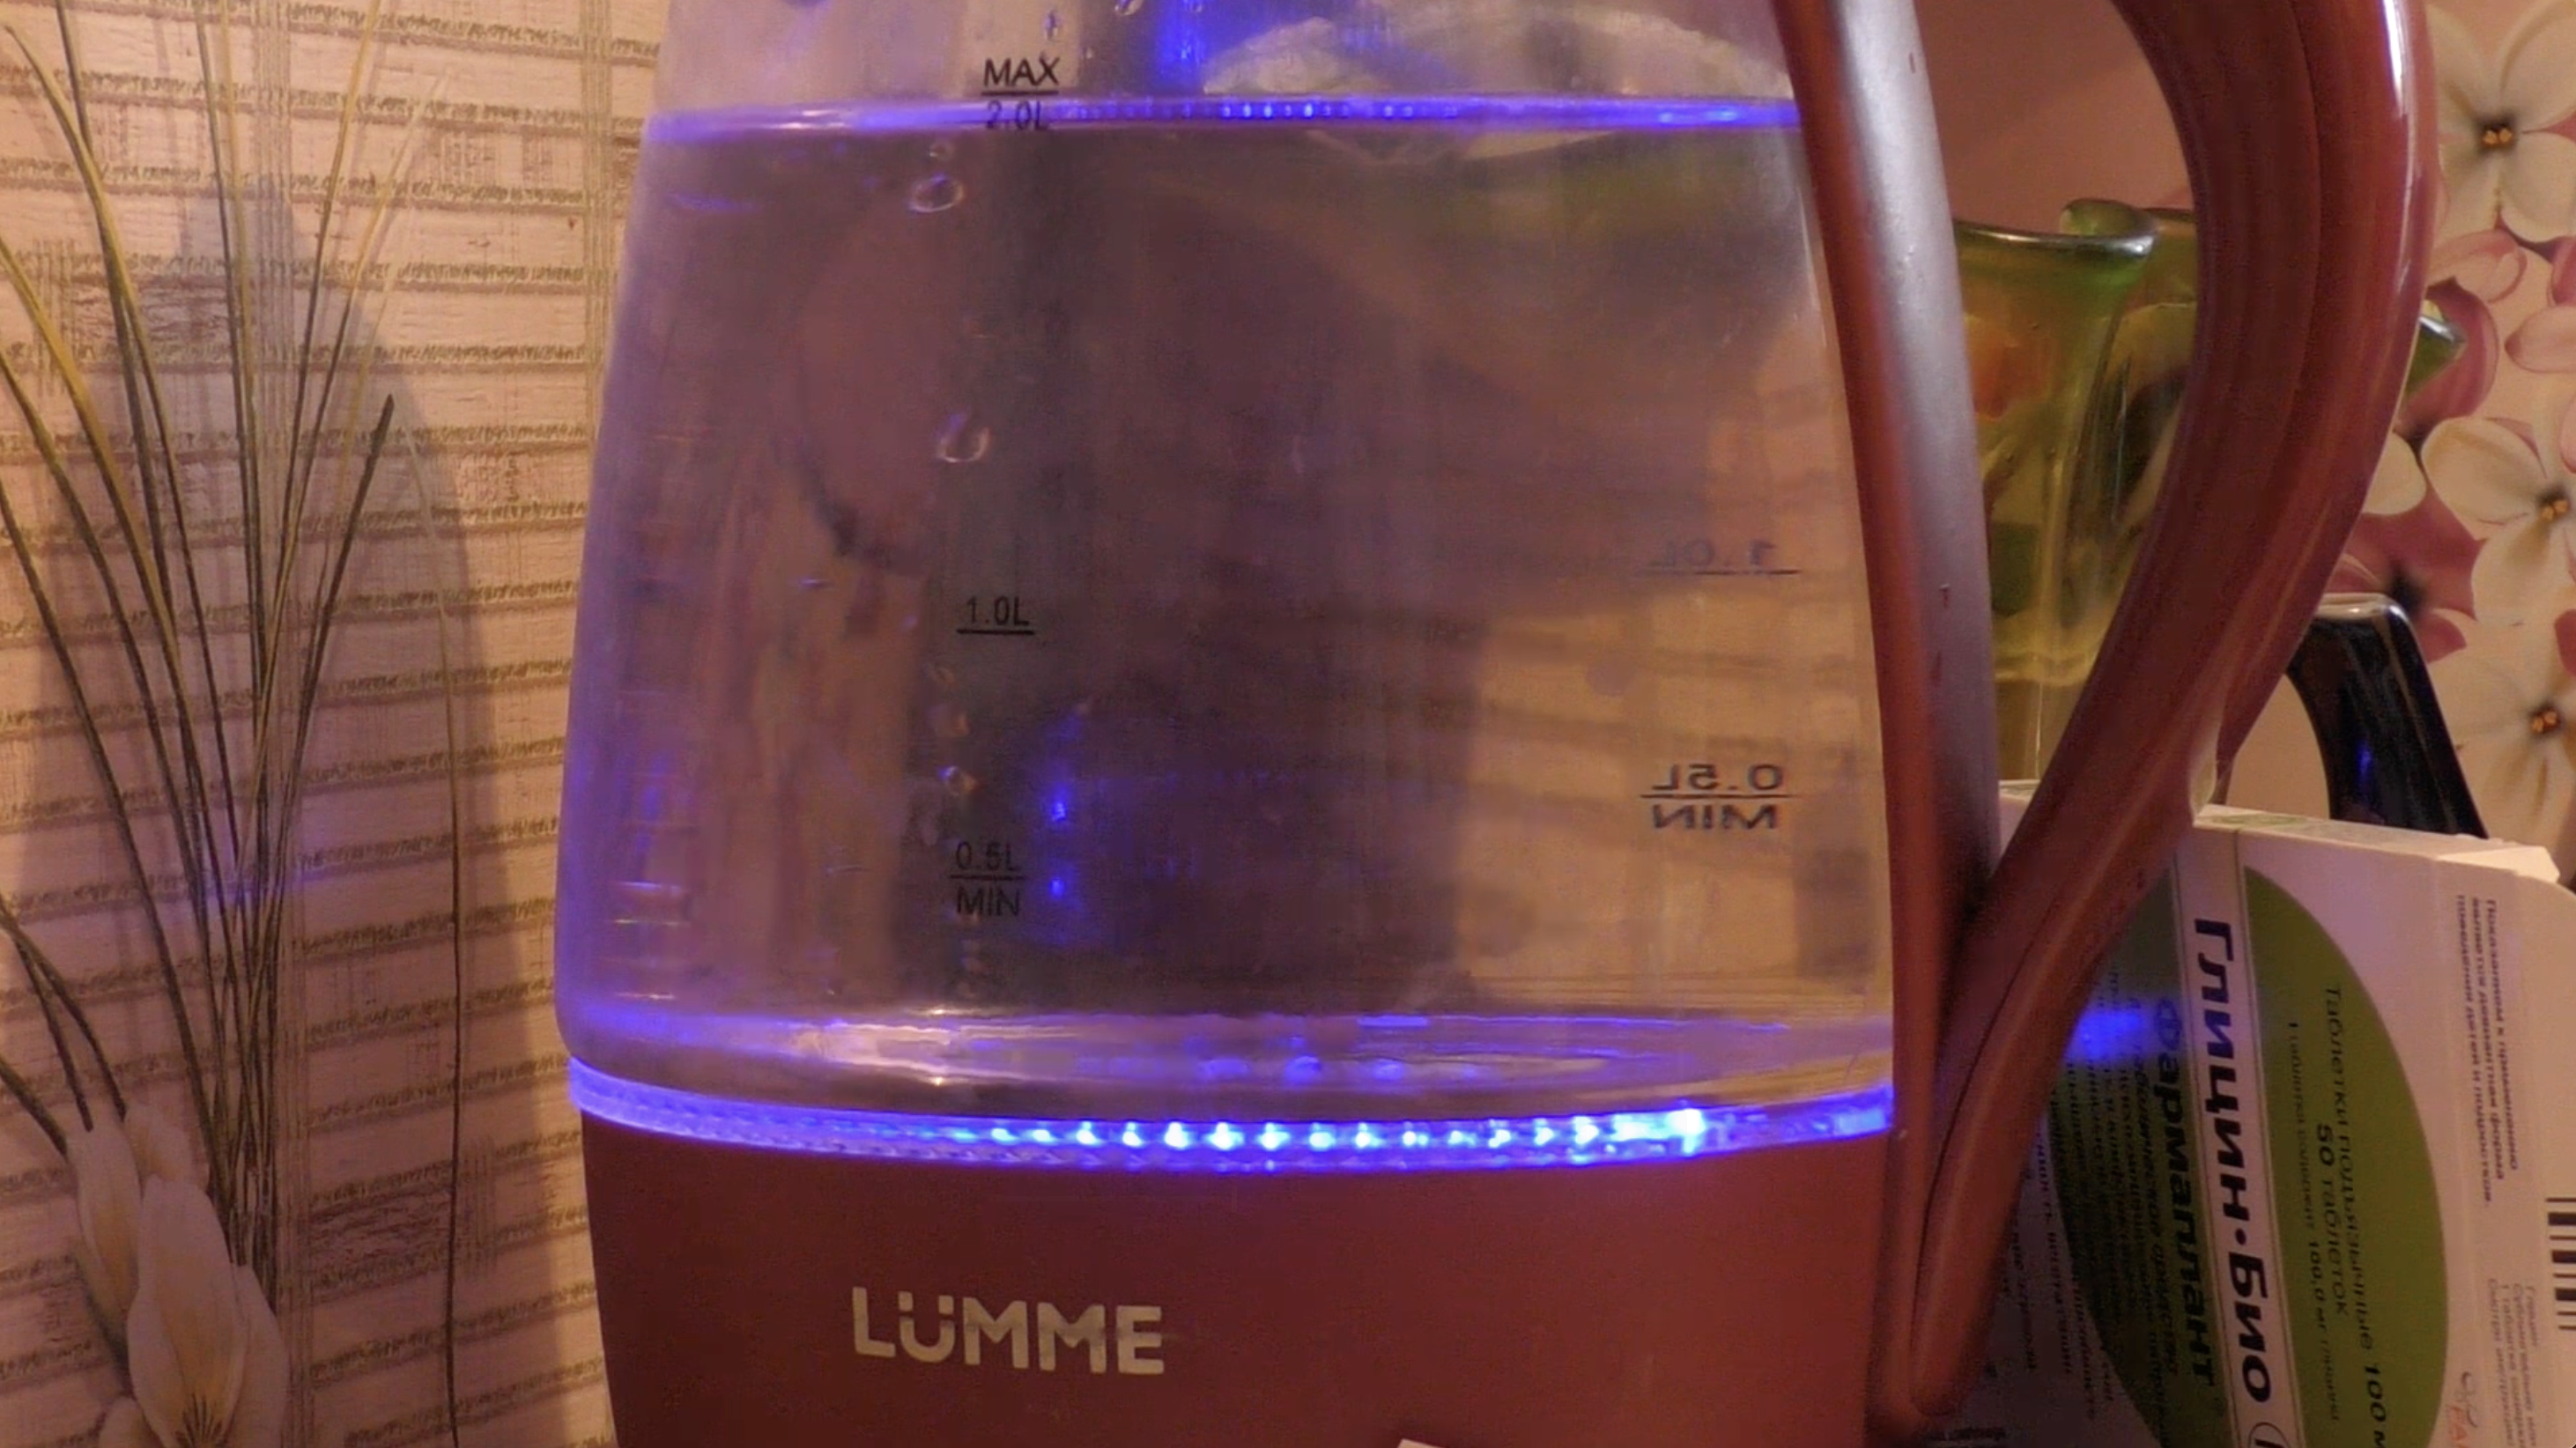
\includegraphics[width=0.7\textwidth]{images/image.png}
	\caption{Диаграмма требований к функциональным возможностям АИС}
\end{figure}
\subsection{Верификация}

Для верификации систем используются такие инструменты, как \textbf{CPN Tools} и \textbf{Rodin}, которые поддерживают моделирование и симуляцию сетей Петри и других формальных моделей.

\begin{figure}[H]
	\centering
	\includegraphics[width=0.6\textwidth]{images/Screenshot 2025-10-15 at 11.14.32.png}
	\caption{Диаграмма связанных ПО, для проектирования АИС}
\end{figure}

\subsection{Отечественное ПО}

Примером отечественного ПО является \textbf{MASIW (ИСП РАН)}, предназначенное для проектирования и верификации бортовых ПАК на основе AADL. Этот инструмент позволяет анализировать ресурсы, интерфейсы и сети, а также генерировать конфигурации для сложных систем, что очень важно в высокотехнологичных отраслях.
\begin{figure}[H]
	\centering
	\includegraphics[width=0.7\textwidth]{images/image copy.png}
	\caption{Отечественное ПО, MASIW (ИСП РАН)}
\end{figure}
\newpage
\section*{Заключение}
\addcontentsline{toc}{section}{Заключение}

В работе последовательно рассмотрены принципы организации, этапы и стандарты жизненного цикла автоматизированных информационных систем, а также средства их проектирования и проверки. Показано, что результативная разработка опирается на системное мышление и поэтапное выполнение работ: от содержательного описания предметной области и бизнес-процессов — к формальной модели, далее к корректно оформленному техническому заданию, пилотированию и промышленному внедрению. Разделение на слои (данные, логика, интерфейс) и поддержание согласованности между ними обеспечивает управляемость изменений и упрощает интеграцию с внешними системами.

Сравнение классического и метамодельного подходов показывает, что классическая схема быстро даёт локальный результат, но дорого обходится при изменении схем данных и масштабировании. Метамодельная инженерия, опирающаяся на метаданные, металлогику и мета-интерфейсы, обеспечивает переиспользование решений, трассируемость артефактов и устойчивость к изменениям требований на всём горизонте жизни системы. Единая терминология между заказчиком, проектировщиком и разработчиком, а также связные модели требований, архитектуры и сценариев поведения снижают риск несоответствий на стыках работ.

Стандарты ISO/IEC 12207 (для программного обеспечения) и ISO/IEC 15288 (для систем) задают полный набор процессов: от соглашений и организационного обеспечения до проектных и технических процедур, включая верификацию, валидацию, сопровождение и списание. Их применение позволяет формализовать управление качеством, конфигурацией и рисками, а также обеспечить воспроизводимость и контролируемость результатов.

Анализ практических ситуаций подтверждает выводы: ERP-внедрения уровня SAP R/3 требуют значительных затрат и длительной адаптации под отраслевую специфику; при высокой уникальности процессов целесообразно рассматривать собственные АСУ. В авиационной тематике раннее архитектурное моделирование (AADL), анализ безопасности и генерация целевых конфигураций (например, под VxWorks 653) позволяют выявлять дефекты на стадии проектирования и сокращать стоимость исправлений.

Инструментальная база поддерживает методологию: средства визуального моделирования (IBM Rhapsody, Sparx EA, Modelio, Eclipse Papyrus) обеспечивают описание архитектуры и трассируемость; формальные средства (CPN Tools, Rodin) — проверку корректности моделей; платформы для исполняемых предметно-ориентированных языков (GEMOC Studio) и отечественные решения (MASIW для AADL) — поддержку сложных и критичных доменов. В совокупности это снижает технические и проектные риски, повышает качество, сопровождаемость и интегрируемость АИС.


\newpage
\addcontentsline{toc}{section}{Список литературы}
\begin{thebibliography}{9}

    \bibitem{Shevchenko201x}
    Шевченко, О.В. \textit{Анализ современных подходов проектирования информационных систем}. — Известия ЮФУ. Технические науки, с. 89–93. % :contentReference[oaicite:0]{index=0}
    
    \bibitem{Nazarova201x}
    Назарова, О.Б. \textit{Реализация процессов жизненного цикла сложных автоматизированных систем на основе стандартов программной инженерии}. — (научная статья, описание стандартов ISO/IEC 12207 и ISO/IEC 15288). % :contentReference[oaicite:1]{index=1}
    
    \bibitem{RogozovFinaev}
    Рогозов, Ю.И.; Финаев, В.И. \textit{Этапы проектирования автоматизированных систем управления}. — Известия ТРТУ. % :contentReference[oaicite:2]{index=2}
    
    \bibitem{Samonov2019}
    Самонов, А.В. \textit{Методы и средства разработки автоматизированных информационных систем на основе онтологии «Управление качеством программно-технических комплексов»}. — Труды ИСП РАН, т. 31, вып. 5, 2019, с. 165–182. DOI: 10.15514/ISPRAS-2019-31(5)-13. % :contentReference[oaicite:3]{index=3}
    
    \end{thebibliography}
    
\end{document}